%%%%%%%%%%%%%%%%%%%%%%%%%%%%%%%%%%%%%%%%%%%%%%%%%%%%%
%                                                   %
%     Penn State Colloquium Poster Template         %
%                                                   %
% Uses Penn State Colloquium class, with options:   %
%                                                   %
% Orientation:                                      %
%     portrait (default), landscape                 %
%                                                   %
% Paper size:                                       %
%     a4paper (default), a0paper, a1paper, a2paper, %
%     a3paper, a5paper, a6paper                     %
%%%%%%%%%%%%%%%%%%%%%%%%%%%%%%%%%%%%%%%%%%%%%%%%%%%%%
\documentclass{../psuposter}
\renewcommand{\templateimagepath}{../} 


%%%%%%%%%%%%%%%%%%%%%%%%%%%%%%%%%%%%%%%%%%%%%%%%%%%%%
%               Package Dependencies                %
%%%%%%%%%%%%%%%%%%%%%%%%%%%%%%%%%%%%%%%%%%%%%%%%%%%%%
\usepackage{natbib}
\usepackage{lipsum}                                % Dummy text
\usepackage[figwidth = 0.98\linewidth]{todonotes}  % Dummy image (and more!)
\usepackage[absolute, overlay]{textpos}            % Figure placement
\usepackage{braket}
\setlength{\TPHorizModule}{\paperwidth}
\setlength{\TPVertModule}{\paperheight}
\setcitestyle{numbers,square}


%%%%%%%%%%%%%%%%%%%%%%%%%%%%%%%%%%%%%%%%%%%%%%%%%%%%%
%                 AUTHOR AND TITLE                  %
%%%%%%%%%%%%%%%%%%%%%%%%%%%%%%%%%%%%%%%%%%%%%%%%%%%%%
\title{Electronic Transport in Strain-Engineered Graphene}
\author{Nadya Mason}
\institute{University of Illinois}


%%%%%%%%%%%%%%%%%%%%%%%%%%%%%%%%%%%%%%%%%%%%%%%%%%%%%
%                  BEGIN DOCUMENT                   %
%%%%%%%%%%%%%%%%%%%%%%%%%%%%%%%%%%%%%%%%%%%%%%%%%%%%%
\begin{document}
\begin{frame}
\begin{columns}[t, totalwidth=\textwidth]
\begin{column}{0.45\textwidth - 1cm}


%%%%%%%%%%%%%%%%%%%%%%%%%%%%%%%%%%%%%%%%%%%%%%%%%%%%%
%                 BLOCK: BIOGRAPHY                  %
%%%%%%%%%%%%%%%%%%%%%%%%%%%%%%%%%%%%%%%%%%%%%%%%%%%%%
    \begin{block}{Speaker Biographic Summary}
    	\begin{center}
    		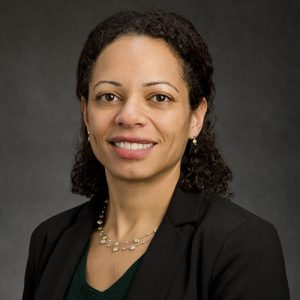
\includegraphics[width=0.75\textwidth]{images/portrait}
    	\end{center}
    	\href{https://publish.illinois.edu/masongroup/}{Dr. Nadya Mason} is the Rosalyn Sussman Yalow Professor in Physics at the University of Illinois Urbana-Champaign. Mason received her bachelor's degree in physics from Harvard University in 1995 and received her doctorate in physics in 2001 from Stanford University, working in the group of Aharon Kapitulnik. Her thesis research was on phase transitions in two-dimensional superconductors. Prior to joining the physics faculty at Illinois, Professor Mason was a Junior Fellow in the Society of Fellows at Harvard University, where she collaborated with Professors Charles Marcus and Michael Tinkham on projects related to both carbon nanotubes and nanostructured superconductors. Prof. Mason has received numerous  awards, including the NSF CAREER Award, Center for Advanced Study Fellowship, and Maria Goeppert Mayer Award.
    \end{block}


%%%%%%%%%%%%%%%%%%%%%%%%%%%%%%%%%%%%%%%%%%%%%%%%%%%%%
%            BLOCK: RESEARCH INTERESTS              %
%%%%%%%%%%%%%%%%%%%%%%%%%%%%%%%%%%%%%%%%%%%%%%%%%%%%%
    \begin{block}{Research Interests}
        Professor Mason's research at Illinois focuses on how electrons behave in low-dimensional, correlated materials, where enhanced interactions are expected to give novel results. The research is relevant to a variety of technologies, including quantum communication, information storage, and qubit control in quantum computers. 
        \begin{center}
	    	
\includegraphics[width=0.85\textwidth]{images/research}    		
    	
    	\textit{Anisotropic magnetoresistance, topological insulators. \cite{masonMasonGroupResearch}} 
    	\end{center}
    	
    \end{block}
\end{column}
\begin{column}{0.55\textwidth - 1cm}


%%%%%%%%%%%%%%%%%%%%%%%%%%%%%%%%%%%%%%%%%%%%%%%%%%%%%
%                 BLOCK: ABSTRACT                   %
%%%%%%%%%%%%%%%%%%%%%%%%%%%%%%%%%%%%%%%%%%%%%%%%%%%%%
    \begin{block}{Talk Abstract}
    	There is wide interest in using strain-engineering to modify the physical properties of 2D materials, for both basic science and applications. Deformations of graphene, for example, can lead to the opening of band gaps, as well as the generation of pseudo-magnetic fields and novel electronic states. We demonstrate how controllable, device-compatible strain patterns in graphene can be engineered by depositing graphene on corrugated substrates. We discuss several techniques for creating corrugated substrates, focusing on periodic spherical curvature patterns in the form of closely packed nanospheres. We show how the smaller nanospheres induce larger tensile strain in graphene, and explain the microscopic mechanism of this. We also present experimental results demonstrating how a nearly periodic array of underlying nanospheres creates a strain superlattice in graphene, which exhibits mini-band conductance dips and magnetic field effects that depend on the magnitude of induced strain. This control of the strain degree of freedom provides a novel platform both for fundamental studies of 2D electron correlations and for prospective applications in 2D electronic devices.
    \end{block}


%%%%%%%%%%%%%%%%%%%%%%%%%%%%%%%%%%%%%%%%%%%%%%%%%%%%%
%                BLOCK: BACKGROUND                  %
%%%%%%%%%%%%%%%%%%%%%%%%%%%%%%%%%%%%%%%%%%%%%%%%%%%%%
    \begin{block}{Brief Background}
    	 Two-dimensional materials are promising for next-generation electronics, due to their versatile band structure, high mobility, and superior electric field-effect tunability. Prof. Mason's team systematically varied substrate corrugation features to examine the strain mechanisms. This allowed for the study of the evolution of deformation patterns and the magnitude of strain induced in graphene. They used periodic spherical curvature patterns in the form of closely packed nanospheres, which allowed them to  control the diameter thereby tuning the curvature. Prof. Mason's group found  that larger tensile strain is induced in systems with smaller local radius of curvature. \cite{zhangStrainModulationGraphene2018}
    	%\cite{longLocalAxonalConduction2020} 
        \begin{center}
		   	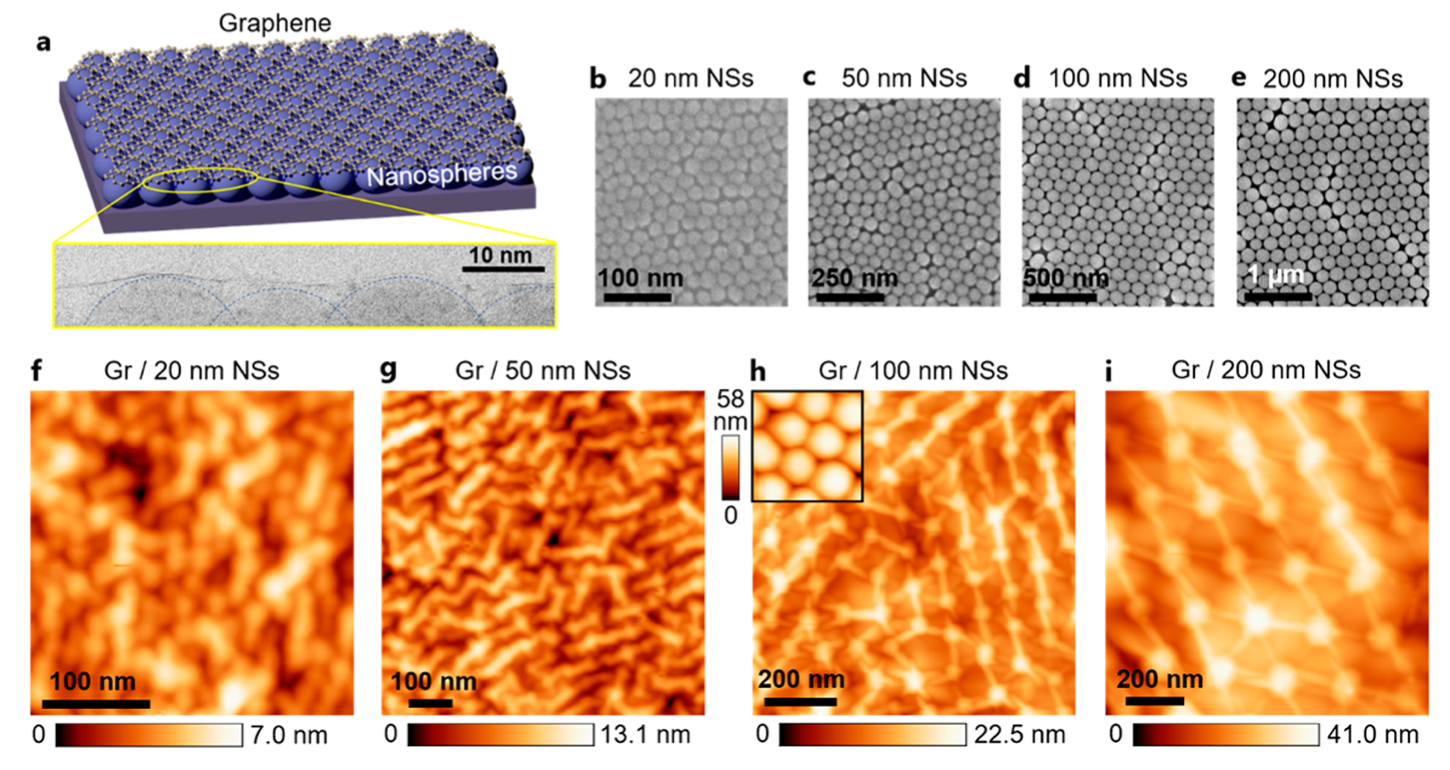
\includegraphics[width=0.8\textwidth]{images/background}    		

		\textit{Structure of the graphene on nanosphere systems. \cite{zhangStrainModulationGraphene2018}}
    	\end{center}
		%\cite{longMorphologicalCharacterizationHVC2018} 
    \end{block}


%%%%%%%%%%%%%%%%%%%%%%%%%%%%%%%%%%%%%%%%%%%%%%%%%%%%%
%                 BLOCK: REFERENCES                 %
%%%%%%%%%%%%%%%%%%%%%%%%%%%%%%%%%%%%%%%%%%%%%%%%%%%%%
\nocite{*}
    \begin{block}{References}
        \bibliographystyle{aipnum4-1}
%        \bibliographystyle{iopart-num}
		\bibliography{references}
    \end{block}

\end{column}
\end{columns}


%%%%%%%%%%%%%%%%%%%%%%%%%%%%%%%%%%%%%%%%%%%%%%%%%%%%%
%                    FOOTER TEXT                    %
%%%%%%%%%%%%%%%%%%%%%%%%%%%%%%%%%%%%%%%%%%%%%%%%%%%%%
\begin{textblock}{0.5}(0.18, 0.94)
    \color{white}
    \sffamily
    \textbf{Eberly College of Science}
    \\
    Department of Physics
\end{textblock}


%%%%%%%%%%%%%%%%%%%%%%%%%%%%%%%%%%%%%%%%%%%%%%%%%%%%%
%                   END TEMPLATE                    %
%%%%%%%%%%%%%%%%%%%%%%%%%%%%%%%%%%%%%%%%%%%%%%%%%%%%%
\end{frame}
\end{document}
